\subsection{Comparison at a Common Calibration Budget}
\label{sec:recovery-comparison}
On a separate cohort, the nominal bank and the continuous
generalized likelihood ratio (GLR) observer used the same nominal
operators, eight PMUs, source catalog and permitted startup prefix. The
GLR carries one committed state through restoration. ExtraTrees was
refitted on disjoint simulated parents covering the same catalog.
A common publication clock and calibration procedure selected a
threshold for each arm under a normal-alarm budget of one per hour.
The fixed methods were then scored once on \RecParents{} event parents
and \RecNormalParents{} normal parents. Interventions did not overlap,
and the next onset was 3--8\,s after physical restoration.

\begin{figure*}[t]\centering
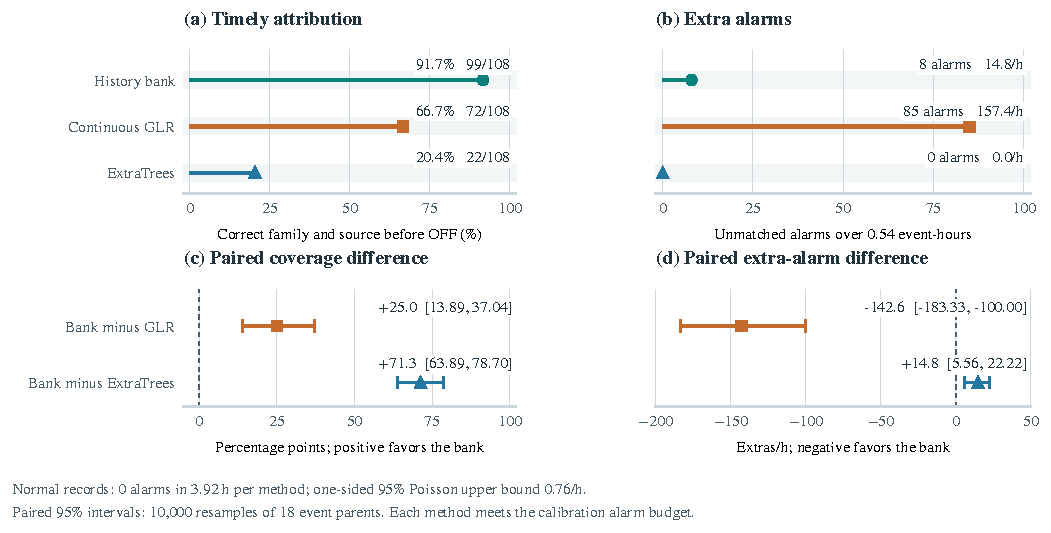
\includegraphics[width=.99\textwidth]{figures/generated/recovery_comparison_c02.pdf}
\caption{Coverage and alarm cost on held-out sequences. (a) Correct family
and source reported before OFF, out of 108 interventions. (b) Unmatched alarms
on event records, with rates per monitored event-hour. (c) History-bank coverage minus each comparator, computed with 10,000 paired resamples of the
18 event parents. Positive values favor the bank. Thresholds were selected
on separate calibration data under a target of one normal alarm/h. All three
methods emitted zero alarms in 3.92 normal hours each; the one-sided 95\%
Poisson upper bound is 0.76/h.}
\label{fig:recovery-c02}\end{figure*}

Figure~\ref{fig:recovery-c02} shows a \RecGlrDiff{} percentage
point gain over GLR (paired 95\% CI \RecGlrCI), with fewer extra alarms.
The gain over ExtraTrees is \RecTreesDiff{} points (95\% CI
\RecTreesCI), with more extra alarms. The intervals resample entire
physical parents within the network/noise strata; events within a
parent do not count as independent samples. All three methods had zero
normal alarms in \RecNormalHours{} monitored hours per method (one-sided
95\% Poisson upper bound: \RecNormalUpper{}/h). The result is conditional
on the count model and the aggregate exposure. The two physical methods
differ in candidate search, score semantics and commitment, so the
comparison does not isolate the effect of explicit recovery histories.
